% Full instructions available at:
% https://github.com/elauksap/focus-beamertheme

\documentclass{beamer}
\usepackage[UTF8]{ctex}
\usepackage{amsmath}
\usepackage{amssymb}
\usepackage{tikz}
\usepackage{booktabs}
\usepackage{multirow}
\usepackage{color,xcolor}

\usetheme{focus}

\definecolor{bl}{HTML}{b33939}
\definecolor{rh}{HTML}{009432}
\definecolor{aq}{HTML}{F0E7DA}
\definecolor{rs}{HTML}{A6B4B3}
\definecolor{ln}{HTML}{2980b9}
\definecolor{r}{HTML}{ff3838}

\title{2.2.1 椭圆及其标准方程}
% \subtitle{Subtitle}
\author{杨习}
\titlegraphic{\includegraphics[scale=0.2]{myLogo.png}}
\institute{shineyoung7@163.com}
\date{2018.12.12}

\begin{document}

    \begin{frame}
        \maketitle
    \end{frame}

    \section{复习}
    \begin{frame}{\qquad 圆的知识内容}
        \begin{itemize}
          \item \textcolor{ln}{圆的定义:}\pause 平面内,到\alert{一个定点} 的\textcolor{example}{距离等于定长}的所有的点的轨迹. \pause
          \item \textcolor{ln}{如何画一个圆?}\pause
          \item \textcolor{ln}{圆的标准方程:}\pause $ (x-a)^2+(y-b)^2=r^2 $
        \end{itemize}\pause
        \begin{block}{思考一下:}
          平面内,到\alert{两个定点的距离之和}等于\alert{定长}的点的轨迹又是什么呢?
        \end{block}

        %     \item \textcolor{ln}{为了得到圆的标准方程,我们先做了一件什么事呢?}\pause
        %   \end{itemize}
        %   \column{0.4\textwidth}
        %   \begin{tikzpicture}[scale = 0.7]
        %     \draw[->] (-2,0) -- (2,0)node[right]{$x$};
        %     \draw[->] (0,-2) -- (0,2)node[above]{$y$};
        %     \draw[color=ln,line width=1pt] (0,0) circle(1.5);
        %     \node[below=7pt,left] at (0,0) {$o$};
        %   \end{tikzpicture}
        % \end{columns}
        %
        %   \begin{itemize}
        %     \item \textcolor{ln}{建立圆的平面直角坐标系遵循了什么原则呢?}\pause

    \end{frame}

    \begin{frame}{\qquad 知识目标}
      \begin{enumerate}
        \item 理解椭圆的缘之所起
        \item 能通过自己的动手操作,深层次理解椭圆是什么
        \item 会由椭圆的定义推出椭圆的标准方程
      \end{enumerate}
    \end{frame}

    \section{引入}

    \begin{frame}{\qquad 中国国家大剧院}
      \includegraphics[scale=0.25]{e1.jpg}
    \end{frame}
    \begin{frame}{\qquad 天体运行轨道}
      \centering
      \includegraphics[scale=0.18]{e2.jpg}
    \end{frame}


    \section{如何画一个椭圆?什么是椭圆?}

    \begin{frame}{\qquad 如何画一个椭圆?}
      \begin{columns}
        \column{0.6\textwidth}
        小实验材料:\\ 草稿纸、针管笔、细绳、图钉. \pause \vspace{15pt}

        步骤:\pause
        \begin{enumerate}
          \item 取出不可拉伸的定长细绳;在草稿纸上画两个定点$F_1, F_2$;\pause
          \item 将细绳的两端固定在这两个定点上;\pause
          \item 用笔尖把细绳拉紧,在草稿纸上慢慢移动,画出一条轨迹,观察画出的图形. \pause
        \end{enumerate}

        \column{0.4\textwidth}
          \includegraphics[scale=0.04]{e3.jpg}
      \end{columns}

    \end{frame}

    \begin{frame}
      \begin{block}{思考}
        \begin{enumerate}
          \item 在画轨迹的过程中,细绳两端的位置是固定的 还是运动的?\pause \\ \alert{细绳两端处于定点上} \pause
          \item 在画轨迹的过程中,轨迹上的点始终满足一个什么条件?
        \pause \\ \alert{轨迹上的点到两定点的距离之和始终不变} \pause
          \item 在画轨迹的过程中,细绳的长度和两定点的距离 有怎样的大小关系?\\ \alert{细绳长度 $>$ 两定点距离}
        \end{enumerate}
      \end{block}\pause
      由此,大家能通过这一小实验归结出\textcolor{rh}{椭圆的定义}了吗?
    \end{frame}

    \begin{frame}{\qquad 什么是椭圆?}
      \begin{alertblock}{椭圆的定义}
        平面内,到\alert{两个定点}$F_1, F_2$ \pause 的\alert{距离之和}\pause 等于\alert{常数}\pause \textcolor{rh}{(大于$|F_1F_2|$)}\pause 的点的轨迹叫做椭圆. \pause
      \end{alertblock}
      \begin{block}{一些定义}
        \begin{itemize}
          \item 两个定点$F_1, F_2$ —— \textcolor{ln}{焦点}; \pause
          \item 两个焦点之间的距离$|F_1F_2|$ —— \textcolor{ln}{焦距} \pause
        \end{itemize}
      \end{block}
    \end{frame}

    \begin{frame}{\qquad 椭圆定义辨析}
      \begin{block}{思考}
        平面内,到\textcolor{rh}{两定点} \alert{距离之和} 等于 \alert{常数} 的点的轨迹都是\alert{椭圆}吗?
      \end{block} \pause
      \vspace{10pt}
      若距离之和$(|MF_1| + |MF_2|)$ 为常数:\pause
      \vspace{10pt}
      \begin{itemize}
        \item 距离之和 \alert{$>$} 焦距:\pause 轨迹为\alert{椭圆};\pause
        \item 距离之和 \alert{$=$} 焦距:\pause 轨迹为一条\alert{线段$F_1F_2$};\pause
        \item 距离之和 \alert{$<$} 焦距:\pause 轨迹\alert{不存在}.
      \end{itemize}
    \end{frame}

    \begin{frame}{\qquad 椭圆定义辨析}
      \begin{block}{练一下}
        已知$A(-3.0), B(3,0)$, 点$M$到$A, B$ 两点的距离之和为 $2a$:
        \begin{enumerate}
          \item 当$2a=10$ 时,点$M$ 的轨迹是什么?\pause \alert{椭圆};
          \item 当$2a=6$ 时,点$M$ 的轨迹是什么?\pause \alert{线段AB};
          \item 当$2a=5$ 时,点$M$ 的轨迹是什么?\pause \alert{没有轨迹};
        \end{enumerate}
      \end{block}
    \end{frame}

    \section{椭圆的标准方程}

    \begin{frame}{\qquad 建立椭圆的平面直角坐标系}
      建立平面直角坐标系通常遵循的原则:\alert{对称、简洁}\pause

      \begin{columns}[onlytextwidth]
          \column{0.5\textwidth}
          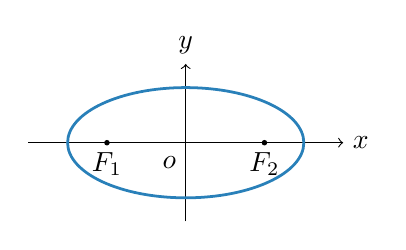
\begin{tikzpicture}
            \draw[->] (-2,0) -- (2,0)node[right]{$x$};
            \draw[->] (0,-1) -- (0,1)node[above]{$y$};
            \draw[color=ln,line width=1pt] (0,0) ellipse [x radius=1.5cm, y radius=0.7cm];
            \fill (-1,0)node[below]{$F_1$} circle (1pt);
            \fill (1,0)node[below]{$F_2$} circle (1pt);
            \node[below=7pt,left] at (0,0) {$o$};
          \end{tikzpicture} \pause
          \column{0.5\textwidth}
            以$F_1, F_2$ 所在直线为$x$轴\\ \pause
	          以线段 $F_1F_2$ 的中垂线为$y$轴\\ \pause
	          则线段 $F_1F_2$ 的中点就为原点\\
	          建立平面直角坐标系.

      \end{columns}

    \end{frame}

    \begin{frame}{\qquad 椭圆的平面直角坐标系}

      \begin{columns}[onlytextwidth]
          \column{0.6\textwidth}
          在此,我们设定: \\
          椭圆上的点到焦点的\alert{距离之和}为"\alert{$2a$}"\\ \pause
           \alert{焦距}为"\alert{$2c$}". (且\alert{$2a > 2c > 0$})\pause

          \column{0.4\textwidth}
          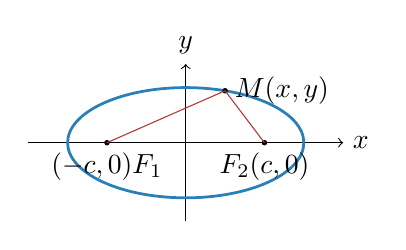
\begin{tikzpicture}
            \draw[->] (-2,0) -- (2,0)node[right]{$x$};
            \draw[->] (0,-1) -- (0,1)node[above]{$y$};
            \draw[color=ln,line width=1pt] (0,0) ellipse [x radius=1.5cm, y radius=0.7cm];
            \fill (-1,0)node[below]{$(-c,0)F_1$} circle (1pt);
            \fill (1,0)node[below]{$F_2(c,0)$} circle (1pt);
            \fill (0.5,0.66)node[right]{$M(x,y)$} circle (1pt);
            \draw[color=bl] (-1,0)--(.5,.66);
            \draw[color=bl] (1,0)--(.5,.66);
          \end{tikzpicture}
      \end{columns}

      那么椭圆上的点到焦点的\alert{距离之和} \textcolor{rh}{等于} \alert{常数} 这样一个几何关系可以转换成一个怎样的数学语言呢?\pause
      \[ |MF_1|+|MF_2|=2a \] \pause
      \[ \sqrt{(x+c)^2+y^2} + \sqrt{(x-c)^2+y^2} = 2a \] \pause
      \begin{block}{思考}
        上式该如何化简呢?
      \end{block}

    \end{frame}

    \begin{frame}{\qquad 求椭圆的标准方程}
        \[ \sqrt{(x+c)^2+y^2} + \sqrt{(x-c)^2+y^2} = 2a \] \pause \vspace{7pt}
        移项,再平方,$ (\sqrt{(x+c)^2+y^2})^2 = (2a - \sqrt{(x-c)^2+y^2})^2 $ \\ \vspace{7pt} \pause
        整理得,$ a^2-cx = a\sqrt{(x-c)^2+y^2} $, \vspace{7pt}\\ \pause
        两边再平方,化简,即得:
        \[ \frac{x^2}{a^2} + \frac{y^2}{a^2-c^2} = 1 \] \pause
        % 由椭圆定义知,$a>c$, 故 $ a^2-c^2 > 0 $. \\ \pause
        设 $ a^2-c^2 = b^2 (b>0) $, \pause 则上式变为:
        \[ \alert{\frac{x^2}{a^2} + \frac{y^2}{b^2} = 1} \]
    \end{frame}

    \begin{frame}{\qquad 椭圆的标准方程}

      \begin{columns}[onlytextwidth]
          \column{0.6\textwidth}
          \begin{alertblock}{焦点在$ x $轴上的 椭圆的标准方程}
            \[ \alert{\frac{x^2}{a^2} + \frac{y^2}{b^2} = 1}(a>b>0) \]
          \end{alertblock}
          \column{0.4\textwidth}
          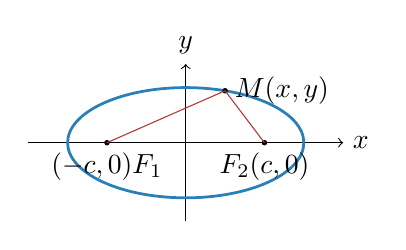
\begin{tikzpicture}
            \draw[->] (-2,0) -- (2,0)node[right]{$x$};
            \draw[->] (0,-1) -- (0,1)node[above]{$y$};
            \draw[color=ln,line width=1pt] (0,0) ellipse [x radius=1.5cm, y radius=0.7cm];
            \fill (-1,0)node[below]{$(-c,0)F_1$} circle (1pt);
            \fill (1,0)node[below]{$F_2(c,0)$} circle (1pt);
            \fill (0.5,0.66)node[right]{$M(x,y)$} circle (1pt);
            % \node[below=7pt,left] at (0,0) {$o$};
            \draw[color=bl] (-1,0)--(.5,.66);
            \draw[color=bl] (1,0)--(.5,.66);
          \end{tikzpicture}
      \end{columns}\pause

      \begin{block}{注意事项}
        \begin{itemize}
          \item 椭圆的焦点在 \pause $x$轴上; \pause
          \item 焦点坐标为: \pause $F_1(-c,0), F_2(c,0)$; \pause
          \item $a^2=b^2+c^2$.
        \end{itemize} \pause
      \end{block}
      \begin{block}{思考}
        若椭圆的焦点在$y$轴上,则其标准方程又是怎样的呢?
      \end{block}

    \end{frame}

    \begin{frame}{\qquad 椭圆的标准方程}

      \begin{columns}[onlytextwidth]
          \column{0.6\textwidth}
          \begin{alertblock}{焦点在$ y $轴上的 椭圆的标准方程}
            \[ \alert{\frac{y^2}{a^2} + \frac{x^2}{b^2} = 1}(a>b>0) \]
          \end{alertblock}
          \column{0.4\textwidth}
          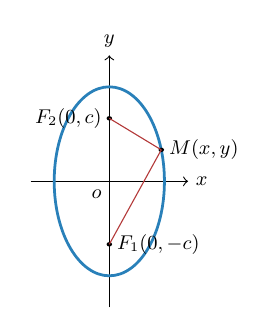
\begin{tikzpicture}[yscale=0.8]
            \tikzstyle{every node}=[font=\small,scale=0.8]
            \draw[->] (-1,0) -- (1,0)node[right]{$x$};
            \draw[->] (0,-2) -- (0,2)node[above]{$y$};
            \draw[color=ln,line width=1pt] (0,0) ellipse [x radius=0.7cm, y radius=1.5cm];
            \fill (0,-1)node[right]{$F_1(0,-c)$} circle (1pt);
            \fill (0,1)node[left]{$F_2(0,c)$} circle (1pt);
            \fill (0.66,0.5)node[right]{$M(x,y)$} circle (1pt);
            \node[below=6pt,left] at (0,0) {$o$};
            \draw[color=bl] (0,-1)--(0.66,0.5);
            \draw[color=bl] (0,1)--(0.66,0.5);
          \end{tikzpicture}
      \end{columns}\pause

      \begin{block}{注意事项}
        \begin{itemize}
          \item 椭圆的焦点在 \pause $y$轴上; \pause
          \item 焦点坐标为: \pause $F_1(0,c), F_2(0,-c)$; \pause
          \item $a^2=b^2+c^2$.
        \end{itemize}
      \end{block}

    \end{frame}

    \begin{frame}{\qquad 椭圆的标准方程}
      \begin{columns}
        \column{0.5\textwidth}
        \begin{alertblock}{焦点在$ x $轴}
          \[ \alert{\frac{x^2}{a^2} + \frac{y^2}{b^2} = 1}(a>b>0) \]
        \end{alertblock}
        \column{0.5\textwidth}
        \begin{alertblock}{焦点在$ y $轴}
          \[ \alert{\frac{y^2}{a^2} + \frac{x^2}{b^2} = 1}(a>b>0) \]
        \end{alertblock}
      \end{columns}
      \begin{exampleblock}{特别注意:}
        \begin{itemize}
          \item 方程的形式:\pause 左边是两个分式的平方和,右边是"1";\pause
          \item 三个参数$a,b,c$的关系:\pause \alert{$a^2=b^2+c^2$}; \pause
          \item 谁的分母大,焦点就在谁轴上("比大小");
        \end{itemize}
      \end{exampleblock}
    \end{frame}

    \begin{frame}{\qquad 练习:判断椭圆焦点所在轴}

      判断下列椭圆焦点在哪个轴上,并指明$a^2,b^2$, 及其焦点坐标.

      \begin{enumerate}
        \item[(1).] $\frac{x^2}{25} + \frac{y^2}{16} = 1 \qquad$ \pause \textcolor{rh}{在$x$轴上,\pause $(-3,0)$和$(3,0)$. }
        \item[(2).] $\frac{x^2}{144} + \frac{y^2}{169} = 1 \qquad$ \pause \textcolor{rh}{在$y$轴上,\pause $(0,-5)$和$(0,5)$. }
        \item[(3).] $\frac{x^2}{m^2} + \frac{y^2}{m^2+1} = 1 \qquad$ \pause \textcolor{rh}{在$y$轴上,\pause $(0,-1)$和$(0,1)$. }
      \end{enumerate}

    \end{frame}

    % \begin{frame}{\qquad 练习:求椭圆中的$a,b,c$}
    %   \begin{enumerate}
    %     \item 已知椭圆方程:$\frac{x^2}{25} + \frac{y^2}{16} = 1$, 则 $a=$\pause \textcolor{rh}{5}, $b=$\pause \textcolor{rh}{4}, $c=$\pause \textcolor{rh}{3}.
    %     \item 已知椭圆方程:$\frac{x^2}{6} + \frac{y^2}{3} = 1$, 则 $a=$\pause \textcolor{rh}{$\sqrt{6}$},  $b=$\pause \textcolor{rh}{$\sqrt{3}$}, $c=$\pause \textcolor{rh}{$\sqrt{3}$}.
    %     \item 已知椭圆方程:$\frac{x^2}{9} + \frac{y^2}{16} = 1$, 则 $a=$\pause \textcolor{rh}{4}, $b=$\pause \textcolor{rh}{3}, $c=$\pause \textcolor{rh}{$\sqrt{7}$}.
    %   \end{enumerate}
    % \end{frame}

    \begin{frame}{\qquad 总结}
      \pause
      \begin{columns}
        \column{0.5\textwidth}
          $\frac{x^2}{a^2}+\frac{y^2}{b^2}=1 \pause \alert{(a>b>0)}$\\ \pause
          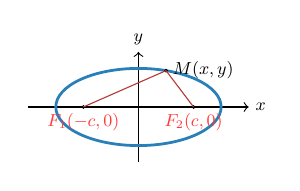
\begin{tikzpicture}[scale=0.7]
            \tikzstyle{every node}=[font=\small,scale=0.7]
            \draw[->] (-2,0) -- (2,0)node[right]{$x$};
            \draw[->] (0,-1) -- (0,1)node[above]{$y$};
            \draw[color=ln,line width=1pt] (0,0) ellipse [x radius=1.5cm, y radius=0.7cm];
            \fill (-1,0)node[color=r, below]{$F_1(-c,0)$} circle (1pt);
            \fill (1,0)node[color=r, below]{$F_2(c,0)$} circle (1pt);
            \fill (0.5,0.66)node[right]{$M(x,y)$} circle (1pt);
            % \node[below=7pt,left] at (0,0) {$o$};
            \draw[color=bl] (-1,0)--(.5,.66);
            \draw[color=bl] (1,0)--(.5,.66);
          \end{tikzpicture}\\ \pause

        \column{0.5\textwidth}
        $\frac{y^2}{a^2}+\frac{x^2}{b^2}=1 \pause \alert{(a>b>0)} $ \\ \pause
        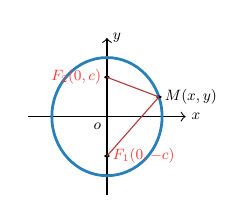
\begin{tikzpicture}[yscale=0.5]
          \tikzstyle{every node}=[font=\small,scale=0.6]
          \draw[->] (-1,0) -- (1,0)node[right]{$x$};
          \draw[->] (0,-2) -- (0,2)node[right]{$y$};
          \draw[color=ln,line width=1pt] (0,0) ellipse [x radius=0.7cm, y radius=1.5cm];
          \fill (0,-1)node[color=r, right]{$F_1(0,-c)$} circle (1pt);
          \fill (0,1)node[color=r, left]{$F_2(0,c)$} circle (1pt);
          \fill (0.66,0.5)node[right]{$M(x,y)$} circle (1pt);
          \node[below=6pt,left] at (0,0) {$o$};
          \draw[color=bl] (0,-1)--(0.66,0.5);
          \draw[color=bl] (0,1)--(0.66,0.5);
        \end{tikzpicture}\\ \pause

      \end{columns}

      \begin{itemize}
        \item \textcolor{ln}{定义:} 平面内,到\alert{两个定点}$F_1, F_2$ \pause 的\alert{距离之和}\pause 等于\alert{常数}\pause \textcolor{rh}{(大于$|F_1F_2|$)}\pause 的点的轨迹\pause \alert{(2a>2c)}. \pause
        \item \textcolor{ln}{$a,b,c$的关系:} \pause \alert{$a^2=b^2+c^2$} \pause
        \item \textcolor{ln}{焦点位置的判断:}\pause 谁的分母大,焦点就在谁轴上\pause \alert{("比大小")}
      \end{itemize}

    \end{frame}

    \begin{frame}{\qquad 拓展练习:求椭圆的标准方程}
      写出适合下列条件的椭圆的标准方程:

      \begin{enumerate}
        \item 焦点坐标为$(0,-4), a=5$; \pause \vspace{20pt}
        \item 焦点在$x$轴上,焦距等于4, 且经过点$P(3,-2 \sqrt{6})$; \pause \vspace{20pt}
        \item $a+c=10, a-c=4$.
      \end{enumerate}
    \end{frame}

    \begin{frame}{\qquad 课后巩固}
      作业:

      《课时作业(八)》
      \vfill
      课后探索:
      \vspace{10pt}

      方程 $Ax^2 + By^2 =1$ 什么时候表示椭圆?

      什么时候表示焦点在 $x$ 轴上的椭圆?

      什么时候表示焦点在 $y$ 轴上的椭圆?

      能表示圆吗?

    \end{frame}

%     \begin{frame}[plain]{Plain frame}
%         This is a frame with plain style and it is numbered.
%     \end{frame}
%
%     \begin{frame}[t]
%         This frame has an empty title and is aligned to top.
%     \end{frame}
%
%     \begin{frame}[noframenumbering]{No frame numbering}
%         This frame is not numbered and is citing reference \cite{knuth74}.
%     \end{frame}
%
%     \begin{frame}{\qquad Typesetting and Math}
%         The packages \texttt{inputenc} and \texttt{FiraSans}\footnote{\url{https://fonts.google.com/specimen/Fira+Sans}}\textsuperscript{,}\footnote{\url{http://mozilla.github.io/Fira/}} are used to properly set the main fonts.
%         \vfill
%         This theme provides styling commands to typeset \emph{emphasized}, \alert{alerted}, \textbf{bold}, \textcolor{example}{example text}, \dots
%         \vfill
%         \texttt{FiraSans} also provides support for mathematical symbols:
%         \begin{equation*}
%             e^{i\pi} + 1 = 0.
%         \end{equation*}
%     \end{frame}
%
%     \section{Section 2}
%     \begin{frame}{\qquad Blocks}
%         \begin{block}{Block}
%             Text.
%         \end{block}
%
%         \begin{alertblock}{Alert block}
%             Alert \alert{text}.
%         \end{alertblock}
%         \pause
%         \begin{exampleblock}{Example block}
%             Example \textcolor{example}{text}.
%         \end{exampleblock}
%     \end{frame}
%
%     \begin{frame}{\includegraphics[scale=0.2]{e.jpg} \qquad Lists}
%         \begin{columns}[t, onlytextwidth]
%             \column{0.33\textwidth}
%                 Items:
%                 \begin{itemize}
%                     \item Item 1
%                     \begin{itemize}
%                         \item Subitem 1.1
%                         \item Subitem 1.2
%                     \end{itemize}
%                     \item Item 2
%                     \item Item 3
%                 \end{itemize}
%
%             \column{0.33\textwidth}
%                 Enumerations:
%                 \begin{enumerate}
%                     \item First
%                     \item Second
%                     \begin{enumerate}
%                         \item Sub-first
%                         \item Sub-second
%                     \end{enumerate}
%                     \item Third
%                 \end{enumerate}
%
%             \column{0.33\textwidth}
%                 Descriptions:
%                 \begin{description}
%                     \item[First] Yes.
%                     \item[Second] No.
%                 \end{description}
%         \end{columns}
%     \end{frame}
% \setbeamertemplate{caption}[numbered]
%     \begin{frame}{\includegraphics[scale=0.2]{e.jpg} \qquad Figures and Tables}
%         \begin{columns}
%             \column{0.4\textwidth}
%                 \begin{figure}
%                     \centering
%                     \includegraphics{focuslogo.pdf}
%                     \caption{Figure caption.}
%                     \label{fig:focuslogo}
%                 \end{figure}
%
%             \column{0.6\textwidth}
%                 \begin{table}
%                     \centering
%                     \begin{tabular}{rcc}
%                          & Heading 1 & Heading 2 \\\hline
%                         Row 1 & \(v_{11}\) & \(v_{12}\) \\
%                         Row 2 & \(v_{21}\) & \(v_{22}\) \\
%                         Row 3 & \(v_{31}\) & \(v_{32}\) \\
%                     \end{tabular}
%                     \caption{Table caption.}
%                     \label{tab:demo}
%                 \end{table}
%         \end{columns}
%     \end{frame}
%
%     \begin{frame}[focus]
%         Thanks for using \textbf{Focus}!
%     \end{frame}
%
%     \appendix
%     \begin{frame}{\includegraphics[scale=0.2]{e.jpg} \qquad References}
%         \nocite{*}
%         \bibliography{demo_bibliography}
%         \bibliographystyle{plain}
%     \end{frame}
%
%     \begin{frame}{\includegraphics[scale=0.2]{e.jpg} \qquad Backup frame}
%         \usebeamercolor[fg]{normal text}
%         This is a backup frame, useful to include additional material for questions from the audience.
%         \vfill
%         The package \texttt{appendixnumberbeamer} is used not to number appendix frames.
    % \end{frame}
\end{document}
